\documentclass{article}
\usepackage{tikz}
\usepackage{fancyhdr}
\usepackage{graphicx}
\usepackage{hyperref}
\pagestyle{fancy}
\fancyhead[L]{Iris layout header}
\fancyfoot[C]{Iris layout footer \thepage}
\begin{document}
\section*{Final layout fixture}
Text and a \href{https://example.test}{link} occupy the compiled page.
\includegraphics[width=20mm]{layout-image.png}
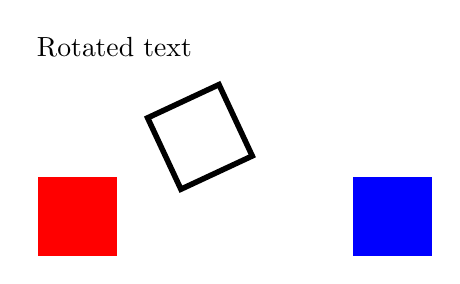
\begin{tikzpicture}
  \fill[red] (0,0) rectangle (1,1);
  \begin{scope}[rotate=25]
    \draw[line width=2pt] (2,0) rectangle (3,1);
    \node at (2,2) {Rotated text};
  \end{scope}
  \begin{scope}
    \clip (4,0) rectangle (5,1);
    \fill[blue] (3,-1) rectangle (6,2);
  \end{scope}
\end{tikzpicture}
\newpage
\section*{Second physical page}
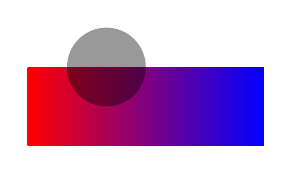
\begin{tikzpicture}
  \shade[left color=red,right color=blue] (0,0) rectangle (3,1);
  \fill[opacity=.4] (1,1) circle (.5);
\end{tikzpicture}
\end{document}
